% XeLaTeX style packages
\documentclass[a4paper,11pt]{article}
%\usepackage[utf8]{inputenc} 
\usepackage{inputenc} 
%\usepackage{fontspec}
%\defaultfontfeatures{Ligatures=TeX}
%\setmainfont{Liberation Serif}
%\usepackage{microtype}
\frenchspacing
\usepackage{enumitem}
\usepackage{color}
\usepackage[top=2cm, bottom=2.5cm, left=2cm, right=2cm]{geometry}
\usepackage{graphicx}
\usepackage{rotating}
\usepackage[binary-units]{siunitx}
\sisetup{range-phrase=--}
\sisetup{range-units=single}
\usepackage{booktabs}
\usepackage{multirow}
%\usepackage[backend=bibtex,sorting=none]{biblatex}
\usepackage[sorting=none]{biblatex}
\bibliography{DUNEPPRP}
%\bibliographystyle{unsrt}
\usepackage{hyperref}
%\usepackage{float}
%\usepackage{subfloat}
%\usepackage{lineno}

\begin{document}
\setcounter{page}{0}
\pagenumbering{Roman}
%\linenumbers

\title{DUNE Construction Proposal}

\begin{center}


\includegraphics[width=\textwidth]{figs/dune-horiz-logo-lg.png}
\vspace{1ex}

{\LARGE\bf 
UK Construction Proposal
}
\vfill

{\bf University of Birmingham:} A.\,Watson

{\bf University of Bristol:} D.\,Cussans, D.\,Newbold, J.\,Rademacker

{\bf University of Cambridge:} A.\,Name

{\bf Daresbury Laboratory:} A.\,Grant

{\bf IPPP, Durham:} S.\,Pascoli

{\bf University of Edinburgh:} D.\,Clarke, F.\,Muheim

{\bf Imperial:} K.\,Long, A.\,Tapper, M.\,Wascko

{\bf University of Lancaster:} A.\,Blake, J.\,Nowak

{\bf University of Liverpool:} C.\,Touramanis

{\bf University of Manchester:} J.\,Evans, S.\,S\"oldner-Rembold, A. Szelc

{\bf University of Oxford:} G.\,Barr, \underline{A.\,Weber}

{\bf Rutherford Appleton Laboratory:} R.\,Preece, C.\,Shepherd-Themistocleous, A.\,Weber, F.\,Wilson

{\bf University of Sheffield:} V.\,Kudryavtsev, N.\,Sooner

{\bf University of Sussex:} C.\,Griffith, J.\,Hartnell, S.\,Peeters

{\bf University College, London:} A.\,Holin, R.\,Nichol

{\bf University of Warwick:} G.J.\,Barker, J.\,Marshall, Y.A\,Ramachers

%{\bf\it full list of academics and project engineers, to be discussed }
\vfill

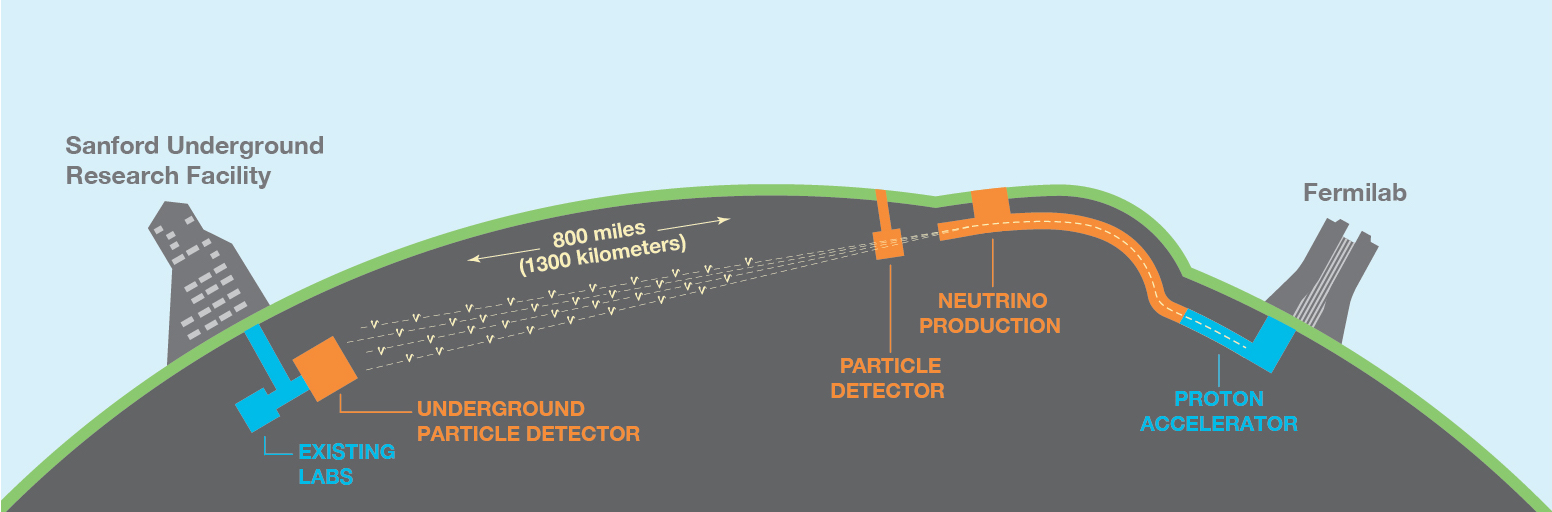
\includegraphics[width=0.9\textwidth]{figs/LBNE_Graphic_061615_2016.jpg}
\end{center}
\vfill

\section*{Summary}
This document is requesting resources and capital for a 7 year construction period in which the DUNE UK collaboration will deliver essential components for the success of the DUNE experiments. The main deliverables will the the Data Acquisition System and 150 Anode Plane Assemblies for two far detector modules, contributions to the software and computing infrastructure, and the preparation for physics exploitation. This is proposal forms part of the overall LBNF/DUNE project proposed in the business case to BEIS.

\thispagestyle{empty}

\newpage
\thispagestyle{empty}
\setcounter{page}{1}

\setcounter{tocdepth}{2}
\tableofcontents
\newpage

\pagenumbering{arabic}

\section{Introduction} 
DUNE is the flagship of the future US domestic particle physics programme and forms a major part of the UK strategy for participation in the next generation of neutrino oscillation experiments. The 1.2\,MW wide-band neutrino beam, generated by the Long Baseline Neutrino Facility (LBNF) at Fermilab, will be fired 1300\,km towards a 40\,kt fiducial mass liquid argon (LAr) time projection chamber (TPC),  located one mile underground at the Sanford Underground Research Facility (SURF) in South Dakota. 

The deployment of this huge LAr detector, illustrated in Figure~\ref{fig:dune:fardet1}, in an intense neutrino beam will represent a game-changing development in the field of neutrino physics. 

\begin{figure}[!htp]
\centerline{
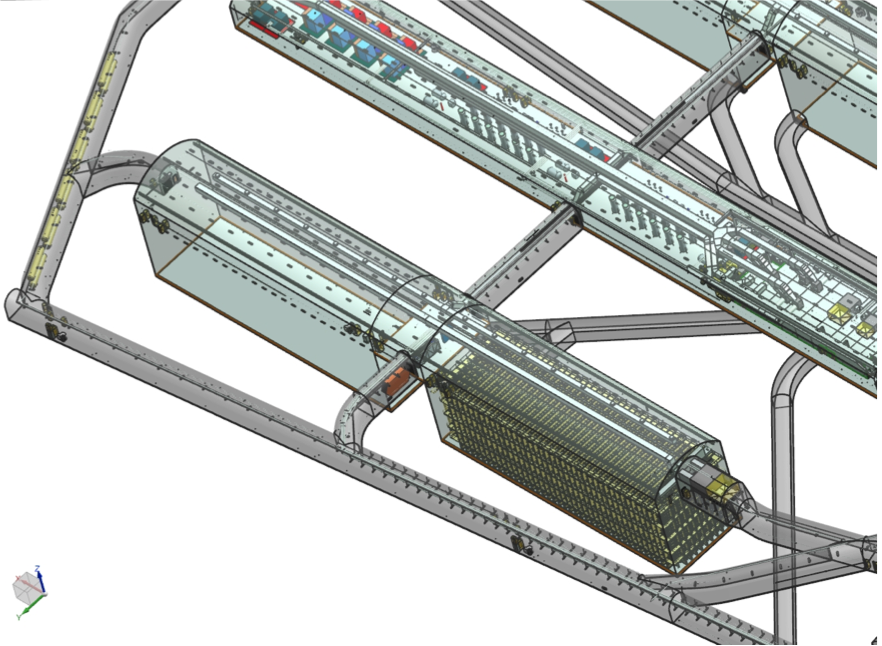
\includegraphics[width=0.5\textwidth]{figs/DUNE_FD.png}
}
\caption[DUNE at SURF]{Illustration of of the underground facility at SURF, showing two of the four underground detector chambers and the central utility cavern. Also shown is the first far detector module (bottom left). To set the scale, the detector chambers are approximately 65\,m long. 
\label{fig:dune:fardet1}}
\end{figure}

In 2014, the US Particle Physics Project Prioritisation Panel (P5) called for the formation of LBNF/DUNE as a truly international project with ambitious scientific goals. LBNF/DUNE was also called out as the highest priority for the US domestic particle physics programme. As a result, the scale and scientific scope of the international LBNF/DUNE project is much greater than that of its predecessor, the US-funded LBNE project. 

LBNF/DUNE was set up as a truly international endeavour from day one -- a first for a US-hosted project of this scale. The international governance model for LBNF and DUNE follows that of the LHC and the LHC experiments. LBNF is the US facility with international contributions at the level of 25\%. DUNE is an international experimental collaboration with an expected US contribution of approximately 25\%. DUNE has broad support from the global particle physics community in the US and Europe and with growing interest in developing countries and Asia. 

LBNF/DUNE passed its DOE CD-1-R review in July 2015, setting the cost for the US contribution at \$1.5B. There is strong support within the US government; both chambers of Congress included authorisation and funding for the LBNF construction start in their FY17 appropriations bills. CD-3a approval for the planned \$300M far site construction was granted in September 2016. This significant milestone marked the approval of the LBNF/DUNE construction, which started in 2017. 

DUNE is strongly supported by CERN who are investing in a large-scale detector prototyping programme at CERN and though a major contribution to the far detector underground facility in South Dakota -- the first time CERN will have invested in an experiment outside CERN. 

While supporting DUNE during the preparatory and pre-construction phases, STFC submitted a business case to BEIS for extra capital and resources to support DUNE, contributions to the facility (LBNF) and the PIP-II accelerator upgrade. The LBNF/DUNE project underwent Gateway Review 0 in the UK, which it passed amber/green. This proposal is putting forward the request for the activities relating to DUNE (WP1-3) as part of the overall LBNF/DUNE project, which also contain the work relating to the target facility (WP4) and the cryo-module for the PIP-II accelerator upgrade (WP5). 

\section{Science Case}
The last 20 years have seen a revolution in our understanding of neutrinos. We now know that neutrinos have mass and the three associated PMNS matrix "rotation" angles have been measured. As it stands, non-zero neutrino masses cannot be accommodated within the Standard Model. Furthermore, the relatively "flat" PMNS neutrino mixing-matrix differs greatly from the near diagonal CKM quark mixing-matrix, possibly providing a window into flavour symmetry. The advancement in our understanding of neutrinos is one of the highlights of recent particle physics, ranking alongside the discovery of a Higgs boson at CERN. 

The latest STFC Programmatic Review recognised this major progress in neutrino physics, but noted that several key science questions remain. 
These crucial open questions include: i) are neutrinos Majorana or Dirac particles; ii) what is the absolute scale of neutrino masses; iii) what is the neutrino mass ordering (MO); and iv) is combined charge and parity (CP) symmetry violated in the leptonic sector? In particular, the observation of CP violation in neutrino oscillations would represent a breakthrough discovery with a potential to explain the matter-antimatter asymmetry in the Universe through the process of leptogenesis. 

\begin{figure}[ht]
    \centering
    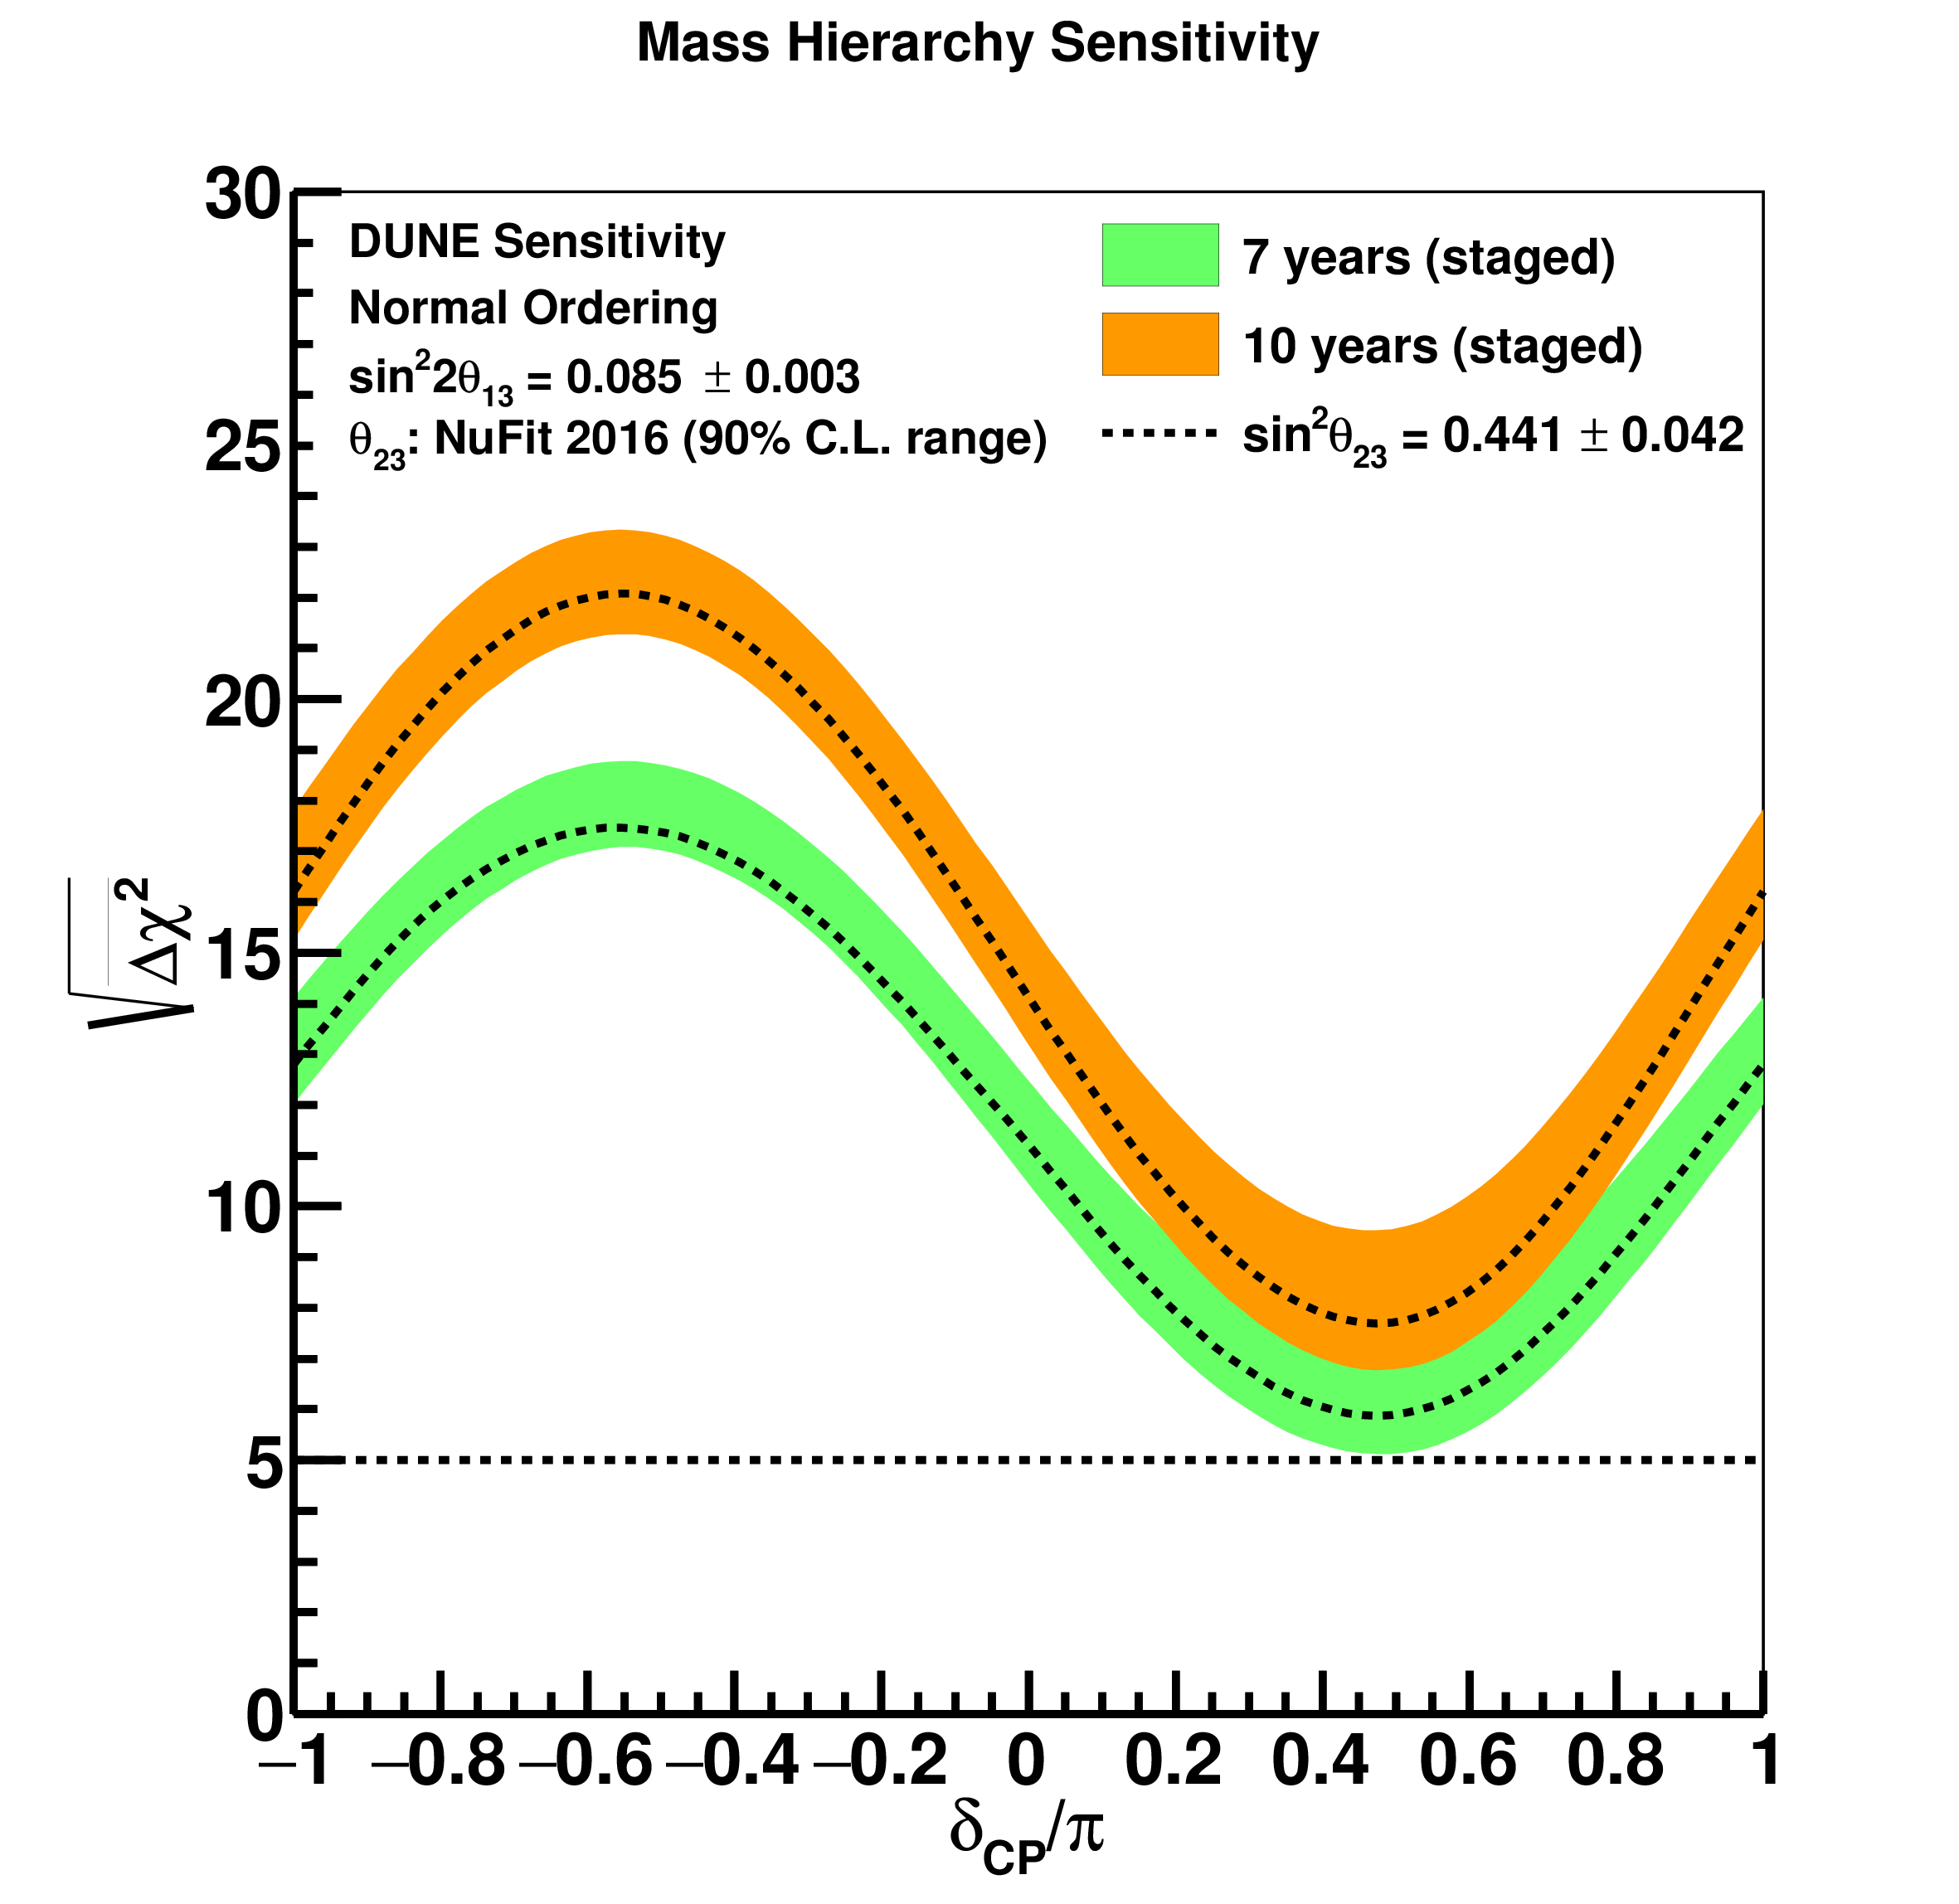
\includegraphics[width=0.47\textwidth]{figs/mh_2017.png}
    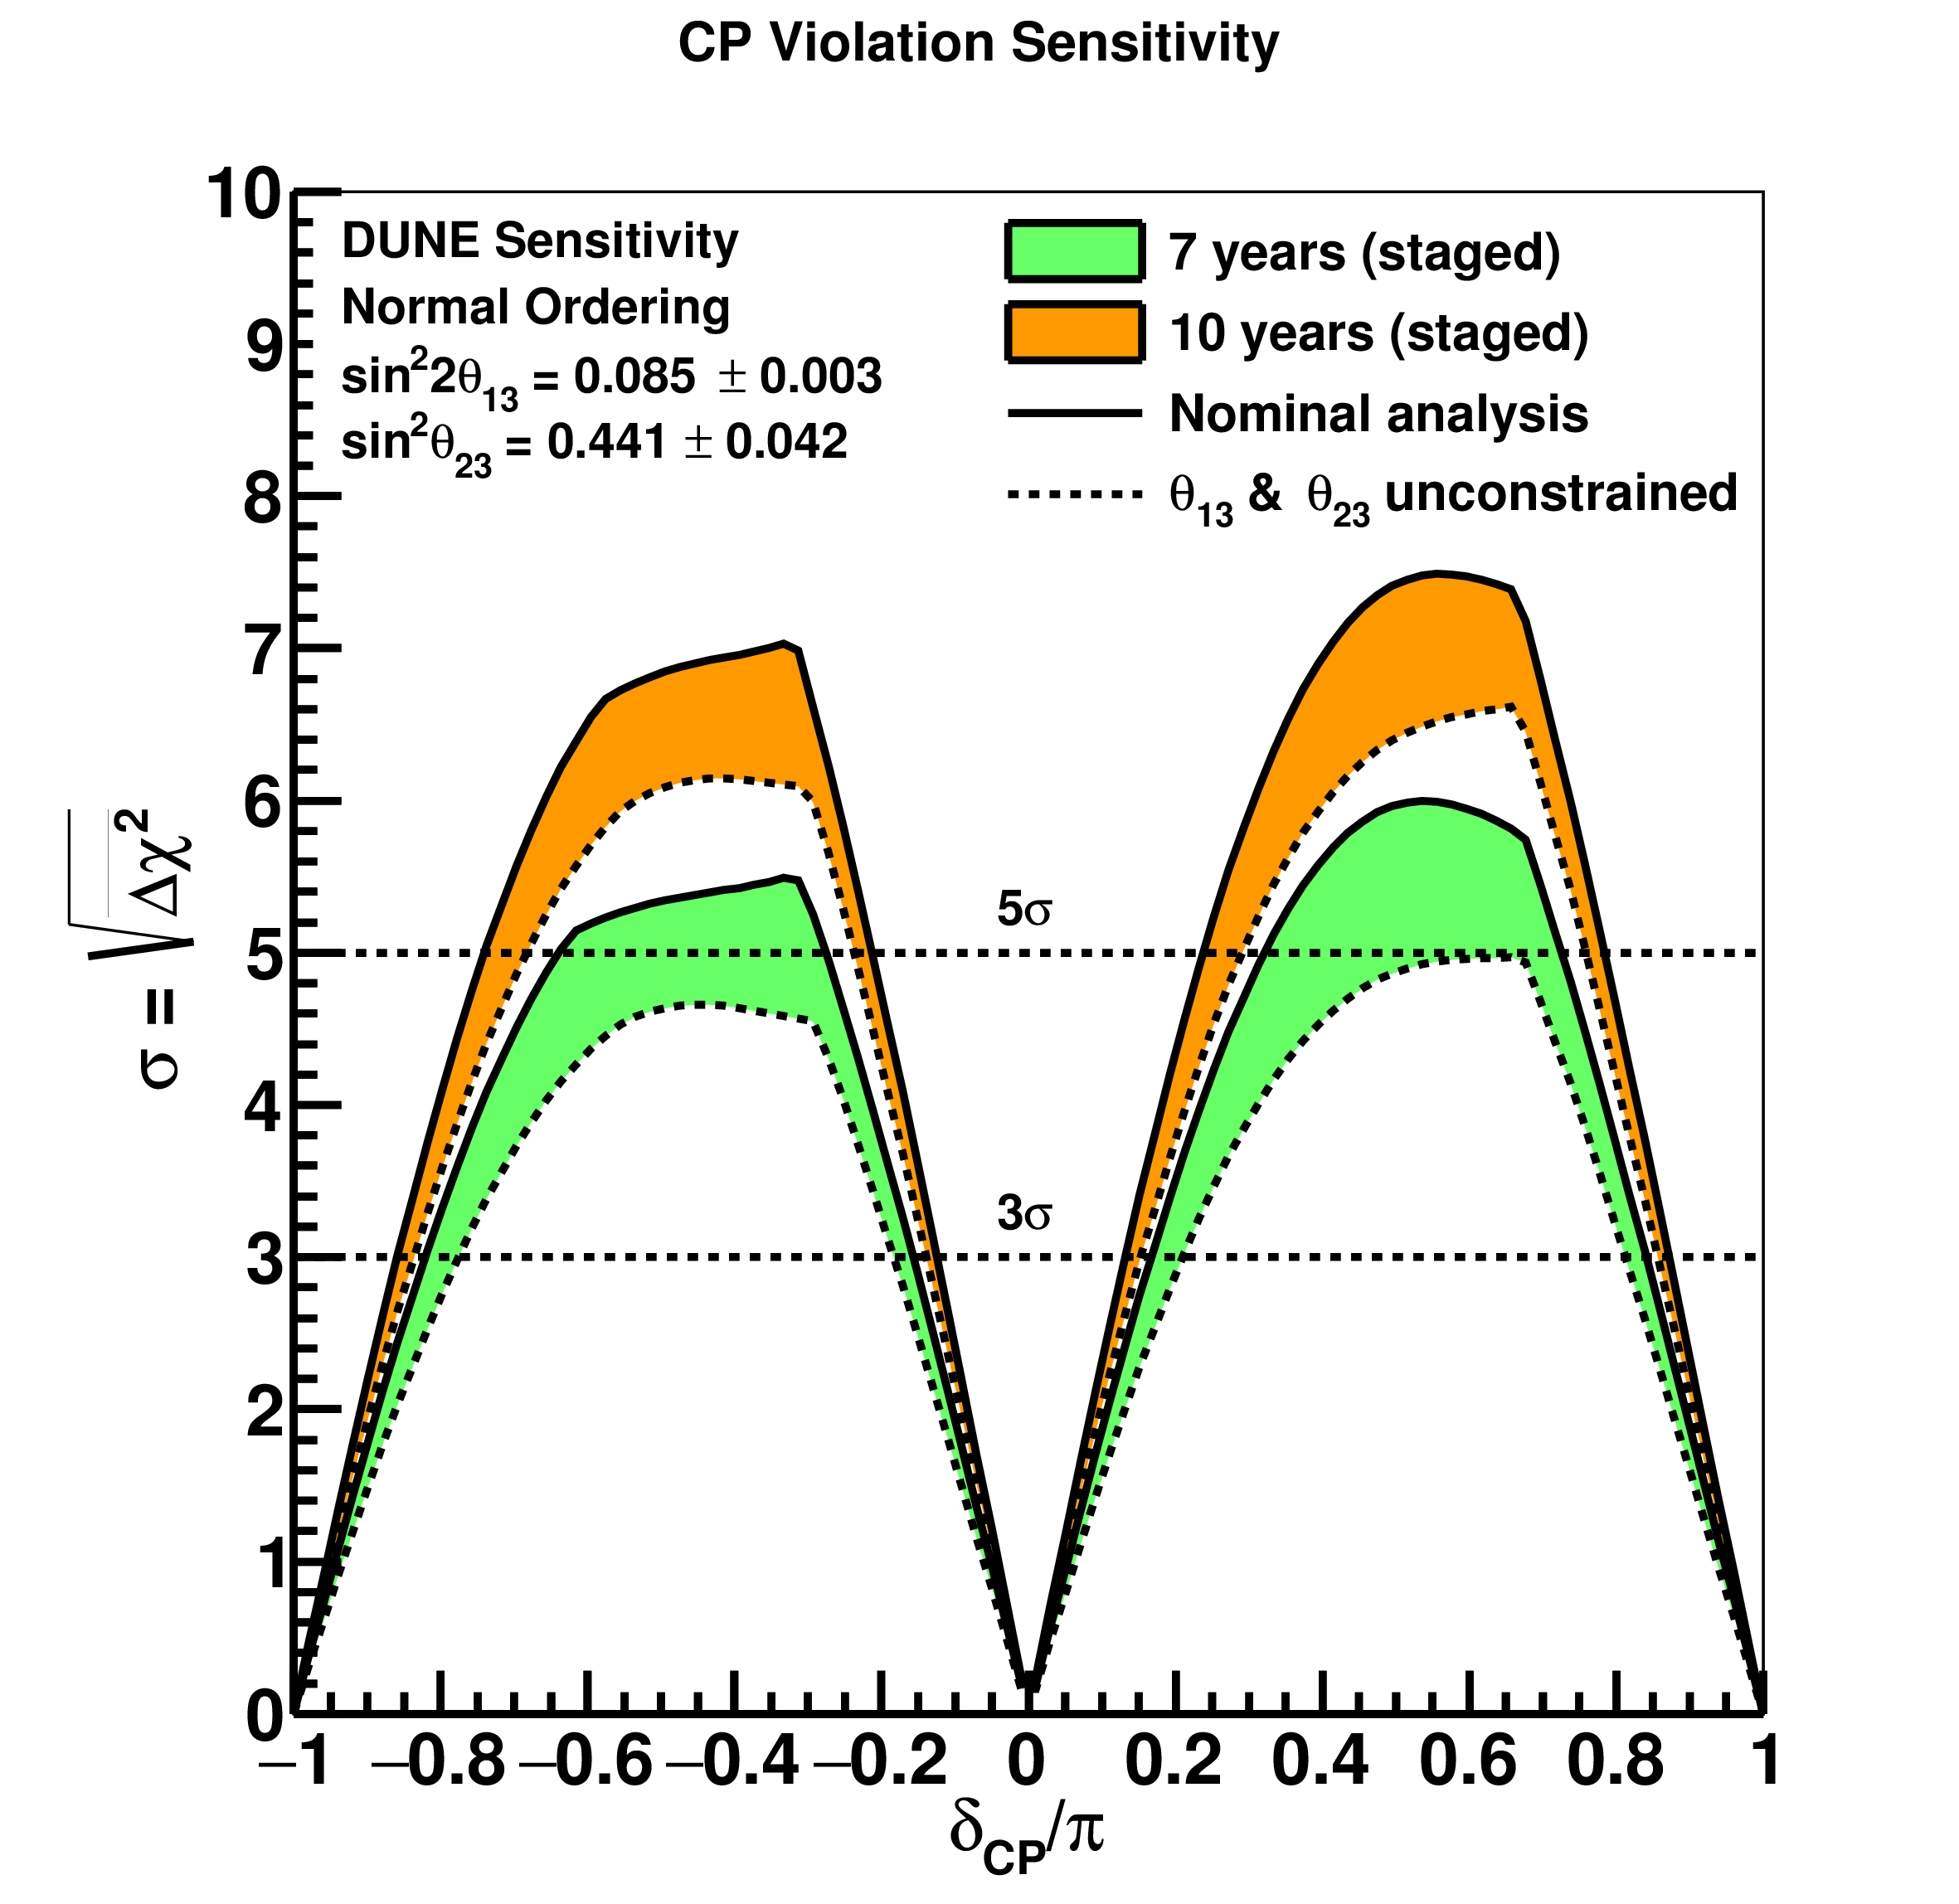
\includegraphics[width=0.47\textwidth]{figs/cpv_2017.png}
    \caption{The plot on the left shows how well DUNE can determine the mass ordering. DUNE will determine the mass ordering independent of the value of all other oscillations parameters with more than 5$\sigma$ after 7 years of running. The right shows the sensitive of how well CP conservation can be excluded as a function of the rue value of $\delta_\text{CP}$ after 7 and 10 years of running.}
    \label{fig:physics}
\end{figure}
 
DUNE will undertake a game-changing programme of neutrino physics, making precision measurements of the parameters that govern $\nu_{\mu} \rightarrow \nu_\text{e}$ and $\overline{\nu}_{\mu} \rightarrow \overline{\nu}_\text{e}$ oscillations. The scientific case for LBNF/DUNE has been presented in detail in volume 2 of the DUNE conceptual design report\cite{2015arXiv151206148D} and only the highest-level scientific goals are repeated here:
\begin{itemize}
\item 
Discovery and measurements of neutrino CP violation. DUNE has $>$3$\sigma$ discovery coverage for 75\% of $\delta_\text{CP}$ values. In favourable regions of parameter space 3$\sigma$ (5$\sigma$) sensitivity can be reached with 3$-$4 (6$-$7) years of operation. Ultimately, $\delta_\text{CP}$ can be measured with a precision of between 7$-$10$^\circ$ (depending on the angle itself), starting to approach the current level for the CP violating angle in the quark sector.   
\item  
Precision neutrino physics, including the definitive determination of the mass hierarchy. Because of the very long baseline, DUNE reaches 5$\sigma$ MO sensitivity within 2$-$5 years 
(depending on the values of other parameters).	
\item
Search for new physics beyond the current understanding of neutrino oscillations. The long-baseline and wide-band neutrino beam will enable DUNE to test the current three-flavour paradigm of neutrino oscillations, providing sensitivity to non-standard neutrino interactions and sterile neutrinos. 
\item 
Observation of the electron neutrino burst from a galactic core-collapse supernova. Unlike in water \v{C}erenkov or liquid scintillator detectors, the main sensitivity in a liquid argon detector is to $\nu_\text{e}$ (rather than $\overline{\nu}_\text{e}$), providing a real-time probe of electron neutrino burst from the initial stage of the neutron star formation phase ($\text{p} + \text{e}^- \rightarrow \text{n} + \nu_\text{e}$). 
\item 
Search for proton decay. Nucleon decay is expected in most models of new physics but has yet to be observed. A large LAr TPC provides an almost background free search for many proton decay modes, including decay modes with kaons.
\end{itemize} 



\section{International Context}
LBNF/DUNE is an approved project with a defined US funding profile. The major milestones through the ten-year construction period are:
\begin{itemize}
     \item {\bf 2017:} start of underground construction at SURF, South Dakota;
     \item {\bf 2018:} operation of the large-scale protoDUNE engineering prototype at CERN; 
     \item {\bf 2019:} provisional international resource matrix for DUNE construction;
     \item {\bf 2019:} technical design report (TDR) for the DUNE detectors (to be reviewed in Q4 2019);
     \item {\bf 2020:} start of production of far detector components;
     \item {\bf 2021:} start of installation the first 10\,kt far detector module at SURF; 
     \item {\bf 2024:} start of physics operation of the first 10\,kt far detector module;
     \item {\bf 2026:} start of 1.2\,MW beam operation with the first two 10\,kt far detector modules.  
\end{itemize}
As of October 2018, the DUNE collaboration consists of around 1100 collaborators from 175 institutions from 31 nations. DUNE/LBNF received strong international support. 

\subsection{Funding Situation}
Only a few countries outside the US have made firm funding commitments towards DUNE/LBNF. But there is a very strong and wide international support and many positive signs from around the world: 
Brazil received R\&D funding from FAPESP; China is providing in-kind contribution to the LBNF beam line; France is funding protoDUNE and large parts for the dual phase detector; Germany received R\&D funding for the near detector and has included it in its future strategy; India has agreed more than \$ 100M of in-kind contribution to PIP-II; Italy has agreed PIP-II contributions and is discussing DUNE involvement; Spain provided R\&D funding for protoDUNE; and Switzerland made a large investment in protoDUNE and is expected to be a major contributor to the near and a Dual Phase far detector.

The funding matrix will be established over the next year in time for CD2. The UK commitment via BEIS was the first of a series of contributions to establish the full funding matrix.


\subsection{Decision Points}

There a some high level decisions, which will influence the UK project. There are two technologies currently considered to be used for the different DUNE FD modules: i) single phase (SP) TPC using the APA readout and ii) dual phase (DP) TPC, which uses Charge Readout Planes (CRPs) in the gas for additional signal amplification. While no formal decision has been made, it is more than likely that the first module will be SP. The formal decision will be made in spring 2019. The second and third modules could be either single or dual phase. The decision on these technologies should be made in time for the DUNE CD2 ({\color{red}give date}) and will depend on the results of running the protoDUNE detectors at CERN and the international funding matrix.

It is likely that at least two SP and one DP modules will be constructed.



\section{Strategy and Objectives (1 page)}
\section{Objectives and Strategy}

The BEIS investment of £65M is to enable the UK to contribute to four key areas of the LBNF and DUNE international construction programme:
\begin{itemize}
    \item PIP-II SRF: The UK will construct and deliver the four high-beta superconducting SRF cavities and assembled cryomodules that make up the final stage of the new PIP-II Linac at Fermilab
    \item LBNF Target: The UK will design, construct and deliver the target for the neutrino beam and elements of the supporting infrastructure, including the complex remote handling system.
    \item DUNE Far Detector:
    \begin{itemize}
        \item DUNE APAs: The UK will construct and deliver 150 of the 300 large (6.0 m x 2.3 m) anode plane assemblies (APAs) for two DUNE Far Detector modules;
        \item DUNE DAQ: the UK will design, construct and deliver the back-end high-speed data acquisition (DAQ) system for two DUNE Far Detector modules.
    \end{itemize}
\end{itemize}
Additionally, the UK is leading the way in the automatic reconstruction of the complex data delivered by the detectors. This is an essential tool which needs further development for the physics exploitation of the experiment.

This investment allows the UK to take a major stake in the DUNE Far Detector construction, securing future access to the best physics for the UK, and to play a leading role in the LBNF beam line and associated PIP-II accelerator development.

The bulk of the UK’s deliverables will be designed and manufactured in the UK, providing opportunities for UK industry to build capability in new and developing technologies, for example, precision engineering, DAQ/electronics, cryogenics and accelerator-based applications. It also offers the possibility to build strong partnerships between UK and developing nations, particularly in Latin America.

The benefits to the UK can be summarised under the following headlines:
\begin{itemize}
    \item Forge a strategic partnership with the US on a high profile international project.
    \item Build a strong partnership between UK and developing nations especially in Latin America.
    \item Industrial engagement with UK industry and capability building.
    \item Skills retention and development of STEM workforce
\end{itemize}

The DUNE UK Construction Project has been structured around the above three main deliverables: preparation for the science, high speed DAQ and APA construction. However, the DUNE collaboration has not made a final decision about the technology to be deployed for different far detector modules. As mentioned earlier, it is generally accepted that the first module will be using the SP technology, while the second and third module could be either SP or DP. Our strategy to deal with this uncertainty is as follows:
\begin{itemize}
    \item We plan to build one half of the APAs for two single phase detectors (150). 
    \item The APA production line would be stopped after 75 APAs, if only one SP detector would be built. The unused capital and resources for the production of the second batch of 75 APAs,
    \todo{Justin, how much would this save?}
    would be come available for the overall LBNF/DUNE project to cover a shortfall of working margin or could be used to change the overall scope of the project. A new proposal would be submitted to STFC to use the saving in such a way as to maximise the return for the UK. These could be one of the following, which have been taken out of the scope of this proposal due to overall capital/resource limitations:
    \begin{itemize}
        \item The UK has developed reflector foil technology, which could be integrated into the cathode plane assembly (CPA). It would increase the overall light level and homogeneity of the system and substantially improve the detector capability for low energy signatures from for example supernova neutrinos.
        \item The has taken a lead in the design of the near detector and is developing the technology for a high pressure gas TPC (HPgTPC), which is very likely to form part of the DUNE near detector complex. We could contribute to construction of a HPgTPC for the near detector.
        \item The exact scope of the WP4 (LBNF target, which is not part of this proposal) has not been defined and is subject to the phase 1 design. Additional resources available from DUNE, could be made available to WP4.
        \item ...\todo{Anything else?}
    \end{itemize}
    \item We plan to deliver the DAQ for one SP and one DP detector. 
    \item The back-end DAQ for both technologies is the same. However, the DP electronics contains functionality that has to be covered by the DAQ in the SP configuration. As such the DAQ for the SP detector is roughly 2 M£ \todo{Giles, is that the right number} more expensive. If the two first detectors are SP, the collaboration as a whole will have to provide the missing resources as the capital/resource limitations of the project do not allow the UK to provide the DAQ for two SP detectors.
\end{itemize}



\section{Project Description}
\subsection{WP0 Management (2 pages)}




\subsection{WP1 Physics (5 pages)}

\subsubsection{Introduction}

Why are we doing this?

test ...

\subsubsection{Work plan}
\subsubsection{WP1.1 Oscillation Physics}
\subsubsection{WP1.2 Reconstruction Software}
\subsubsection{WP1.3 Computing}

\subsubsection{Deliverables and Milestones}

\subsubsection{Business Case}

What are the benefits for the UK?

\subsection{WP2 DAQ (8 pages)}
\subsubsection{WP2.1 A}
\subsubsection{WP2.2 B}
\subsubsection{WP2.3 C}

\subsubsection{Deliverables and Milestones}


\subsection{WP3 APAs (8 pages)}
\subsubsection{WP3.1 A}
\subsubsection{WP3.2 B}
\subsubsection{WP3.3 C}

\subsubsection{Deliverables and Milestones}




\pagebreak

\section{Resource request and Cost}
\section{Resource Request and Cost}

The project cost tables can be found in Appendix \ref{app:A}. Here we summarise the assumption used in deriving the costings.

\subsection{Assumptions in Determining Working Margin}

The working margin (WM) for the project have been determined on a risk based analysis. We have also profiled the WM in time according to when it is most likely needed.

The equipment cost already includes a risk element calculated as follows {\color{red} is this true??? should we separate this out?}
\begin{itemize}
    \item 10\% on equipment for which we have a quote
    \item 20\% on equipment for which we have previous experience
    \item 50\% on equipment for which we have an expert guess
\end{itemize}

\subsection{Costing Assumptions and Methods}

We have used the following assumptions when costing the proposal
\begin{itemize}
    \item This is a capital project, so we assumed that no overhead have to be paid on STFC staff working on WP2/3. 
    \item It is still unclear, if we can recover VAT on equipment to be delivered to the US. We have therefore costed 20\% VAT into all equipment purchase and have included the possible recovery of VAT as a "negative risk" in the risk register.
    \item We make no difference between the traditionally used working allowance (held by the project) and contingency (held by the office) in this project. Instead we are using an overall working margin, which is included in the overall project cost.\footnote{A draft document explaining the use and management of the working margin is available on the TWiki.}
    \item Costs have not been indexed for inflation. However, wage increased due to pay progression have been included.
    \item STFC is only partially funding academics on the consolidated grants. We have therefore used a scaling factor of funded fraction divided by the research time (assumed to be 15\%/60\% for all academics) for their off-project cost, but given their actual FTE involvement in the project.
    \item We have assumed that all STFC staff requested by the collaborating institutions have been awarded, when producing the tables. However, we assigned a substantial WM to account for the fact that these post may not be awarded. (10\% of the fEC, if the person is currently funded on the CG and 80\%, if the person is requested on the CG, but not currently funded on the CG).
    \item ...\todo{What else?}
\end{itemize}

\subsection{Assumptions Relating to Capital}

We have assumed that all cost in WP2 and WP3 can be capitalised except for the WP manager. The WP engineer can be capitalise. We currently assume that the effort going in producing the software asset (PANDORA WP1.1, \todo{WP to be checked}) is resource, but this could be classified as capital as well. We assume the per head part of the CF contribution to be resource, while the equipment levy is capital.


\subsection{Common Fund}

As a recent development, the DUNE collaboration/project requires a construction common fund (CF) to cover the parts of the installation of equipment as well as common infrastructure, which would be difficult for a collaborator to receive funding for. There has been now concrete proposal put forward or agreed at the time of writing this proposal, but the model discussed between the US DUNE/LBNF project and the collaboration is likely to evolve the following assumptions:
\begin{itemize}
    \item Common equipment and infrastructure, which is not part of the facility and which is not easily funded by collaborators is part of the common fund. This could for example include racks, connection between racks and the facility infrastructure, control room, support structure for the APAs, ...
    \item The technical coordination team, in charge of the installation planning, and general purpose technicians and riggers that are needed during the installation are covered by the CF.
    \item The costing model put forward to cover this is suggested to have two components.
    \begin{itemize}
        \item k\$ 7-10 per PhD physicist (or similar) per year over a 5 year period
        \item 10-15\% of the value of core capital contributing to the equipment delivered to DUNE is charged as an additional CF contribution.
    \end{itemize}
    \item it is assumed that CF contributions can be provided in cash or in kind.
\end{itemize}
We have costed our CF contributions at an average level of the above numbers: 8.5k\$ per PhD and year (assuming 100 UK PhD collaborators) and 13\% of the equipment cost. We have informal agreement with the DUNE/LBNF project that this will not change when the real costs have been calculated and agreed by the international Resource Review Board. We also have an agreed set of in-kind contributions, which are listed in WP2 and WP3. The CF contributions\footnote{The exchange rate of 1.2 US\$/1£ has been used.} are summarised in table \ref{tab:CF}.  \todo{(Table needs to be agreed and checked!)}

\begin{table}[htb]
    \centering
    \begin{tabular}{|c||c|c|c|c|c|c|c|c||r|}
        \cline{2-10} \multicolumn{1}{c|}{\ } & \multicolumn{9}{c|}{cost in k£}\\
         \hline
           & 19/20 & 20/21 & 21/22 & 22/23 & 23/24 & 24/25 & 25/26 & 26/27 & total\\
         \hline\hline
         WP2     & & 112 & 112 & 112 & 112 & 112 & & & 560  \\ % 13 of core equipment cost
         WP3     & & 167 & 167 & 167 & 167 & 167 & & & 835  \\ % 13 of core equipment cost
         Per PhD & & 708 & 708 & 708 & 708 & 708 & & & 3,540 \\
         \hline
         total  &  & 987 & 987 & 987 & 987 & 987 & & & 4,935 \\
         \hline\hline
         cash          &     & 492 & 507 & 357 & 642 & 717 &     &     & 2,715 \\ % adjusted to make up total
         WP2 equipment &     & 135 & 135 &     &     &     &     &     & 270 \\ % racks for 2 caverns
         WP1 OC        &     &     &     & 150 & 150 & 150 &     &     & 450 \\ % let's assume 3 years of somebody. too late?
         WP2 TC        & 150 & 225 & 225 & 225 &  75 &     &     &     & 900 \\ %6 years of Tim & TD Eng at 150k£/FTE*y
         WP3 TC        &     & 120 & 120 & 120 & 120 & 120 &     &     & 600 \\ % 4 years of Alan Muir at 150k
         \hline         
         total         & 150 & 835 & 987 & 987 & 987 & 987 &     &     & 4,935 \\
         \hline
    \end{tabular}
    \caption{Breakdown of common fund contributions. The top half of the table shows how much we owe the experiment. The bottom half shows, how we want to cover this with cash and in-kind contributions. It is worth noting that the effort cost in the table are the value of our contributions to the CF, which is higher than the cost to the UK project. For example, the value of an engineering staff year is k\$ 200. }
    \label{tab:CF}
\end{table}



\section{Project Management (8 pages)}
\subsection{Project Governance and Oversight}
\subsection{Change Management}
\subsection{Risk Management}
\subsection{Technical Reviews}
\subsection{Procurement Planning}
\subsection{Benefits Realisation and Impact Planning}
\subsection{QA/QC Planning}
\subsection{Stakeholder engagement and Communications}


\printbibliography
\clearpage


\appendix
\section*{Appendices (no limit)}
\addcontentsline{toc}{section}{Appendices (no limit)}
\renewcommand{\thesubsection}{\Alph{subsection}}

\subsection{Costs by WP and Institution}
\label{app:A}

\newpage

\subsection{Top Level Risks}

\newpage

\subsection{Top Level Milestones and Deliverables}

\newpage

\subsection{Gantt Charts}

\newpage

\subsection{Effort Profiles}

\newpage

\subsection{Key Personnel}
\subsubsection{WP0}

%\noindent
\Dparagraph{Alfons Weber} is the PI of the current DUNE pre-production project and has been the PI and PM of the previous preparatory grant. He has extensive experience in all aspects of accelerator neutrino experiments and has has a long history in their construction and exploitation from MINOS (PMTs, far detector electronics, beam and oscillation analysis convener) over T2K (near detector and electronics convener, cross section convener) and Laguna-LBNO (IB chair) to LBNE/DUNE (UK PI, beam optimisation leader, near detector convener, member of the executive board).

\Dparagraph{Roy Preece} is the current project manager for LBNF/DUNE. He has previously worked as the T2K near detector installation manager in Japan, was in charge of delivering the MICE superconductive magnets and has most recently been the project manager for LZ and the DUNE pre-production project. 
{\color{red}Add his training. Should we mention that he is leaving?}

\Dparagraph{Gary Barker} is deputy PI with special responsibility for the DUNE part of the overall project. He has been a member of T2K and Laguna-LBNO and been in DUNE from the very beginning. He is the chair of the LBNF/DUNE Institutional Board. {\color{red} need to add his experience.}

\subsubsection{WP1}

\Dparagraph{Andy Blake} is awesome and the manager of WP1. He is an expert in the analysis of neutrio data and ...

\Dparagraph{Costas Andreopoulos} is the brain behind GENIE and VaLOR. 

\Dparagraph{John Marshall} is good with computers. brain behind Pandora, 


\Dparagraph{Pete Clarke} knows the GRID

\subsubsection{WP2}

\Dparagraph{Giles Barr} 

\Dparagraph{Simon Peeters} 

\Dparagraph{David Cussans} 

\Dparagraph{An Other} (key technical and management people)


\subsubsection{WP3}

\Dparagraph{\bf Justin Evans} is WP manager

\Dparagraph{\bf Alan Grant} is WP engineer

\Dparagraph{\bf Christos Touramanis} is the consortium leader

\Dparagraph{An Other} (key technical and management people)







\end{document}

